\section{Results and Crosschecks}
\label{sec:TrainClosure}

The analytical solution in Eq.~\eqref{eq:AnalyticSol} sheds a new light onto the
behaviour of the numerical neural network training. In order to study the
training process, the NNPDF collaboration has successfully developed so-called
{\em closure tests}, which we are going to adopt here. 

A closure test uses synthetic data, generated using a known set of PDFs, to
train the neural network. The PDFs used for generating the data are called here
{\em input}\ PDFs. The results of the training are then compared to the known
input PDFs; the performance of the training algorithm and the NN architecture
are assessed by quantifying the comparison between trained PDFs and input PDFs.
Following the original presentation in Ref.~\cite{NNPDF:2014otw}, we distinguish
three levels of closure tests, which are defined by the complexity of the data
used to train the NNs. We use the standard NNPDF nomenclature and refer to these
three levels as level-0 (L0), level-1 (L1), and level-2 (L2) closure tests, and
we denote the input PDFs used to generate the data as $\fin$.

With the full control over the sought solution at hand, the analytic solution
allows us to perform a number of crosschecks that validate our implementation
and provides insight into the training process. These are discussed in the
following sections.


\subsection{Analytical Results and Crosschecks using L0 data}
\label{sec:AnalyticalChecks}
Let us start by discussing the case of L0 closure tests. In this case, the realization
of the dataset is completely determined by the input PDFs, and the values of the data
are given by
\begin{equation}
    \label{eq:DataL0}
    Y_I = T[\fin]_I
        = \sum_{i=1}^{\nflav} \sum_{\alpha=1}^{\ngrid} \FKtab_{Ii\alpha} \fin_{i\alpha}\, ,
\end{equation}
or equivalently, suppressing the indices,
\begin{equation}
    \label{eq:DataL0NoIndices}
    Y = \FKtab \fin\, .
\end{equation}
Note that using L0 data only affects the second term in
Eq.~\ref{eq:AnalyticSol}\footnote{To be more precise, since the analytical
solution is requires the NTK to be frozen at a certain epoch $T_{\rm ref}$, the
NTK will itself depend on the data used in the training.}. We can then rewrite the
combined term in Eq.~\eqref{eq:DataCorrectedInference} as follows
\begin{align}
  \label{eq:TrainingOnLevelZero}
  \check{U}^\perp(t) f_0 + V(t) Y 
    &= \mathcal{M}(t)\, \FKtabT C_{Y}^{-1} \FKtab\, 
      \left[\fin - f_{0}^\parallel\right]\, .
\end{align}
The subtraction taking place in the square brackets of
Eq.~\eqref{eq:TrainingOnLevelZero} suggests us that the effective function that
the neural network actually sees is not the input function $\fin$ used to
generate the data, but rather the difference between $\fin$ and the component of
the initial function $f_0$ that lies in the subspace spanned by the kernel of
the NTK, \ie\ $f_0^\parallel$. In other words, the parallel component
$f_0^\parallel$, which we remind does not evolve during the analytic training,
acts as a constant ``bias'' in the training process, shifting the effective
input function that the neural network sees. Of course the actual magnitude of
this irreducible noise depends both on how $f_0$ and the kernel of the NTK are
distributed over the ensemble. We will come to this point soon.

Note that the observation above remains true even in the limit of infinite training.
This can be shown using
Interestingly, for $t\to\infty$, \ac{How is
this limit justified?} we have
\begin{align}
    \label{eq:LevelZeroClosureInfiniteTraining}
    \lim_{t\to\infty} V(t) Y = \finperp + \mathcal{M}_{\infty} M \finpar
\end{align}
and therefore the $V$ component of the trained solution reproduces exactly the
component of the PDF that lies in  the subspace orthogonal to the kernel of
$\Theta$. We compare the asymptotic behaviour of $V(t) Y$ and $\finperp$ in
Fig.~\ref{fig:InfiniteTimeVterm}.

\begin{figure}[t]
  \centering
  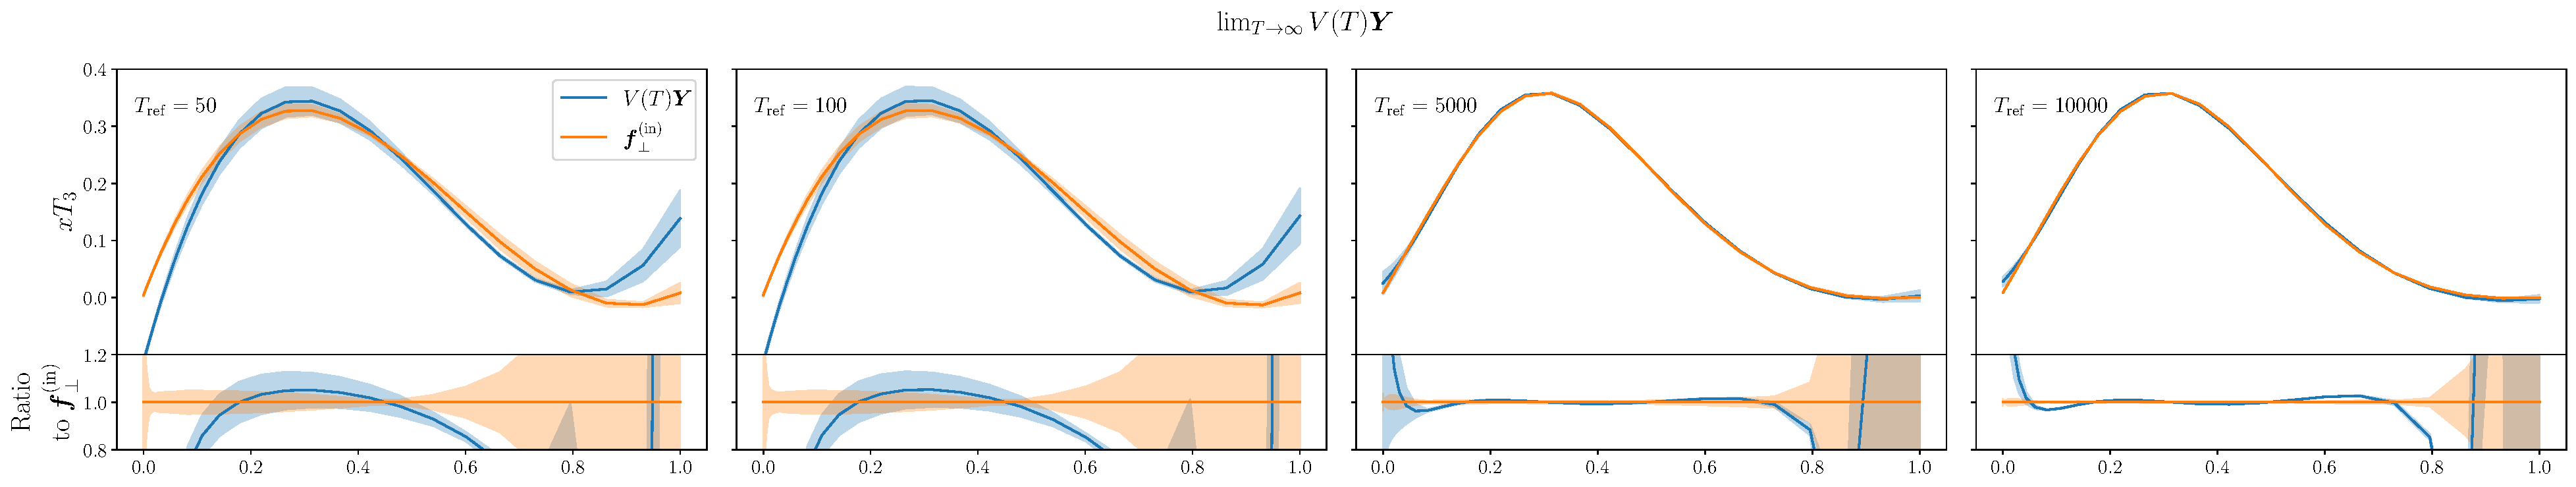
\includegraphics[width=\textwidth]{vy_inf_L0.pdf}  
  \caption{Test the $t\to\infty$ limit of the L0 training for different frozen
  NTK. The orange curve represents the projection of the input function $\fin$
  onto the subspace orthogonal to the kernel of the NTK at $T_{\rm ref}$, \ie\
  $\finperp$. The blue curve represents the contribution of the operator $V$,
  computed with the NTK at $T_{\rm ref}$, in the limit of infinite training
  time.}
  \label{fig:InfiniteTimeVterm}
\end{figure}

The second term in the square bracket on the right-hand side of
Eq.~\eqref{eq:TrainingOnLevelZero} is the contribution from the parallel
component at initialization that does not evolve in the training process. Given
that $f_0$ is almost normally distributed around zero, that term does not
contribute to the central value of the fitted PDF, \ie\ to the average of the
trained solution over replicas. The time evolution of 
\begin{align}
  \label{eq:AverageLevelZeroUcheck}
  \mathbb{E}\left[\mathcal{M}(t)\, \FKtabT C_{Y}^{-1} \FKtab\, 
    f_{0}^\parallel\right]\, ,
\end{align}
is shown in Fig.~\ref{fig:AverageLevelZeroUcheck}.
\begin{figure}[h!]
  \centering
  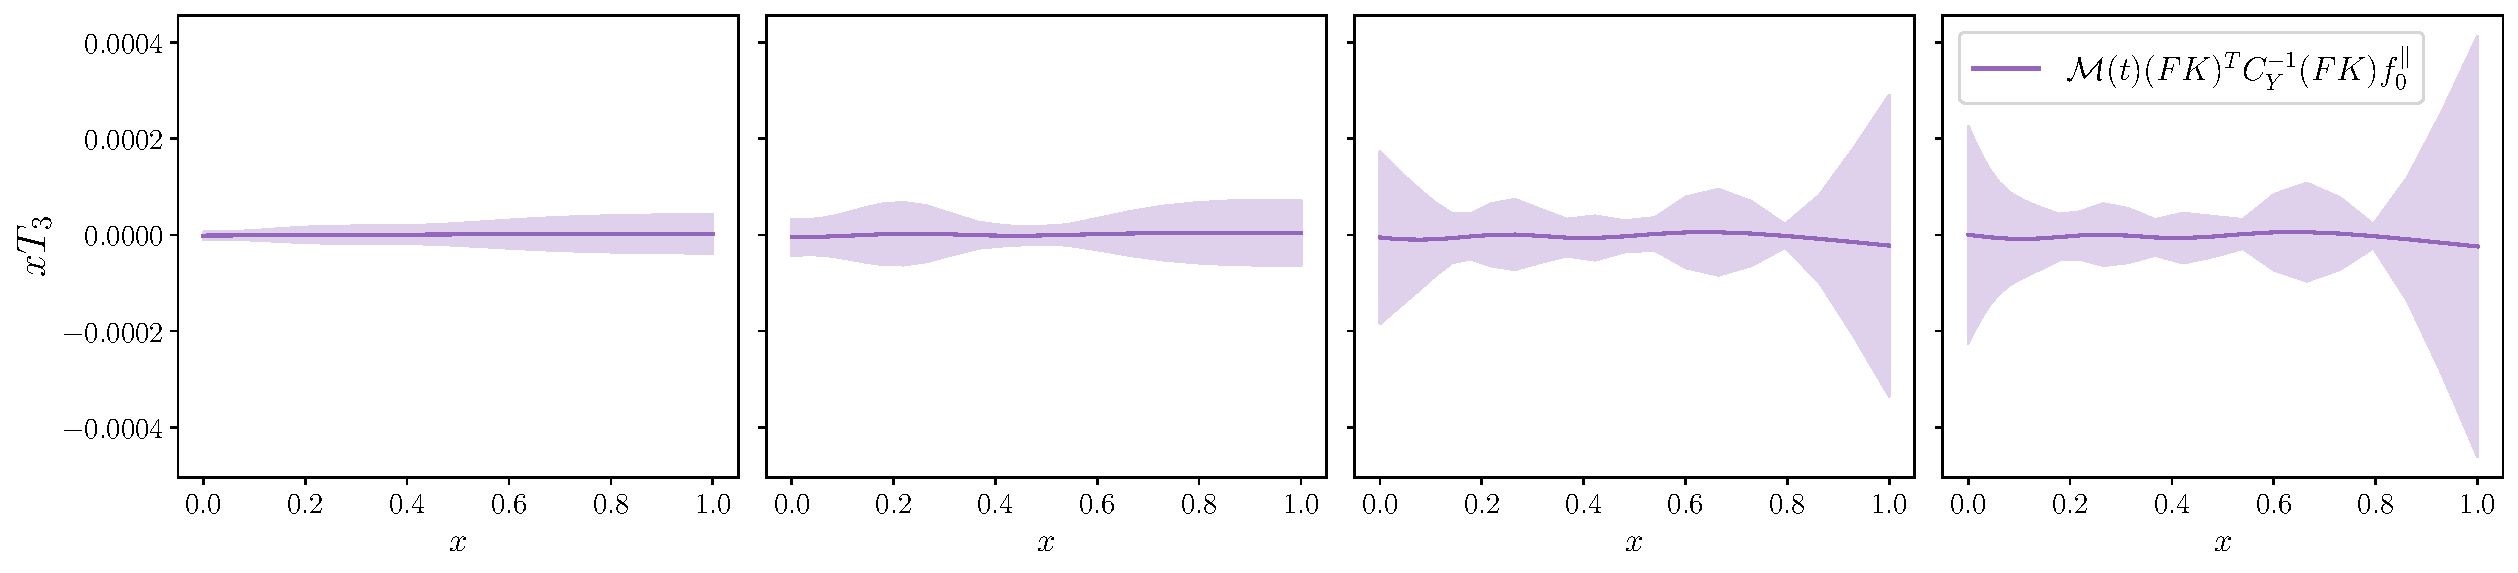
\includegraphics[width=0.95\textwidth]{Mcal_M_fpar_L2_linear.pdf} 
  \caption{Test of the average of the parallel contribution for different
  epochs. The reference epoch at which the frozen NTK is chosen is $T_{\rm ref}
  = 10000$. L2 data is used in the plot.}
  \label{fig:AverageLevelZeroUcheck}
\end{figure}

\FloatBarrier

\subsection{Fluctuations of the Analytical Solution}
\label{sec:CheckCovariance}

In Sect.~\ref{sec:CentralValue} and~\ref{sec:Covariance} we obtained some
simplified expressions for the mean and the covariance of the analytical
solution under the assumption that the fluctuations of the evolution operators
$U(t)$ and $V(t)$ are independent of the fluctuations of the networks at
initialization. Here we quantify this assumption by computing these correlations
explicitly for the dataset and architectures used in this work. In the absence
of general theorems, it is necessary to verify the validity of these assumptions
case by case. The comparison of $\mathbb{E}\left[U(t) f_{0}\right]$ and
$\bar{U}(t) \bar{f}_{0}$ is shown in Fig.~\ref{fig:xT3_exp_val} for $T=20000$.
While the central value of both expressions is compatible with zero, we see that
the fluctuations of $\mathbb{E}\left[U(t) f_{0}\right]$ are much larger than the
ones of $\bar{U}(t) \bar{f}_{0}$, suggesting that using the simplified
expressions results in an incorrect estimate of the error bars. 

\begin{figure}[t!]
  \centering
  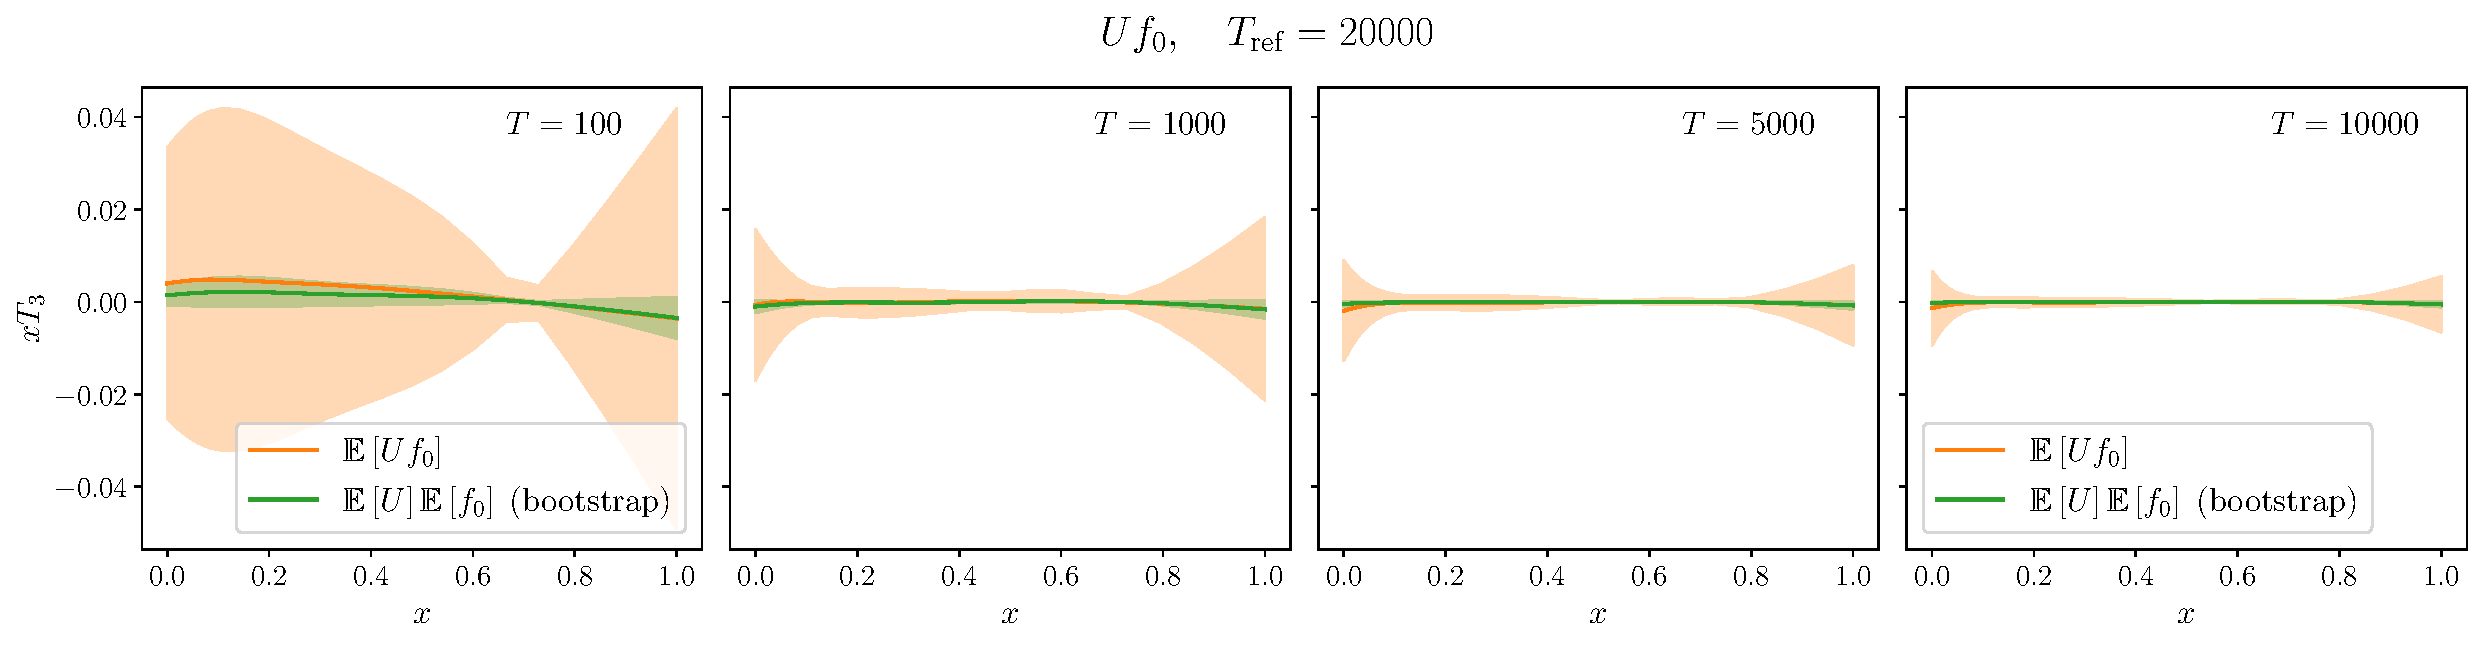
\includegraphics[width=0.95\textwidth]{uf0_L2.pdf}
  \caption{Comparison of $\mathbb{E}\left[U(t) f_{0}\right]$ and $\bar{U}(t)
    \bar{f}_{0}$ as defined in Eqs.~\eqref{eq:MeanValAtT}
    and~\eqref{eq:MeanValAtTNoCorr} respectively, for different epochs $T$. The
    data is obtained by choosing the frozen NTK at $T_{\rm ref} = 20000$, while
    $f_0$ is an ensemble of networks at initialisation (\textit{i.e.}\
    $\mathbb{E}[f_0]=0$). L2 data is used in the plots. \ac{Check correctness of
    bootstrap error with Luigi.}}
    \label{fig:xT3_exp_val}
  \end{figure}
% ===================================

\FloatBarrier

\subsection{Convergence of the Analytical Solution}
\label{sec:CheckAnalyticalConvergence}

At the beginning of the training process there is clearly no difference between
the analytical solution and the trained solution. By construction both AS and TS
are given by the outcome of the neural network at initialization, as discussed
in Sect.~\ref{sec:Init}. In the early stages of training AS and TS differ as
expected. Indeed, the analytical solution is computed using the frozen NTK at
$T_{\rm ref}$, while the trained solution evolves with an NTK that is still
changing as shown in Sect.~\ref{sec:NTKPheno}. Since the NTK at $T_{\rm ref}$ is
already aligned with the solution, the AS converges faster to the target
solution, while the TS takes more epochs before starting to evolve in the right
direction. The two solutions are compared for different training times in
Fig.~\ref{fig:xT3_analytical_vs_trained} after $T=500, 1000$ and 10000 epochs.
The plots in the left column correspond to synthetic L0 data, while the ones in
the right column are obtained using L2 data. The analytical solution is obtained
using a frozen NTK at $T_{\rm ref}=20000$. In both cases the analytical solution
agrees with the trained one for $T=10000$.

  % ===================================
  \begin{figure}[ht!]
    \centering
    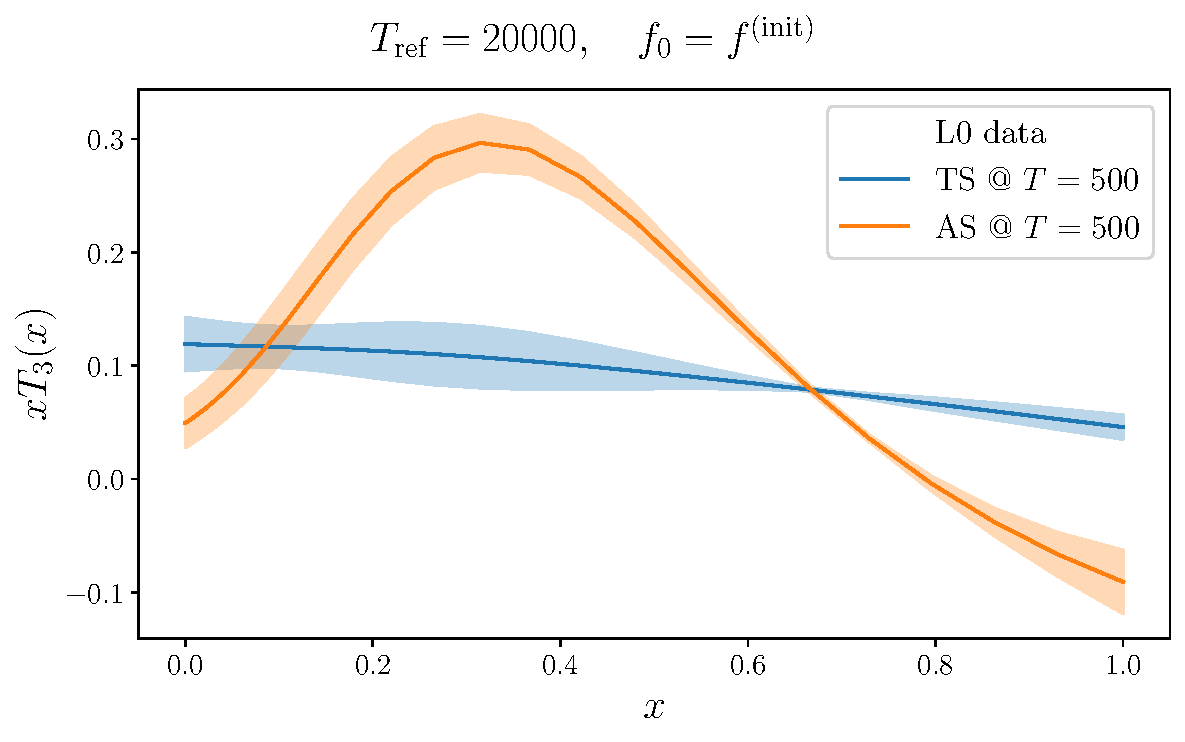
\includegraphics[width=0.45\textwidth]{plots/analytical_solution/xT3/evolution/tr_vs_an/L0/linear/evolution_vs_trained_epoch_500_L0_linear.pdf}
    \hspace{10mm}
    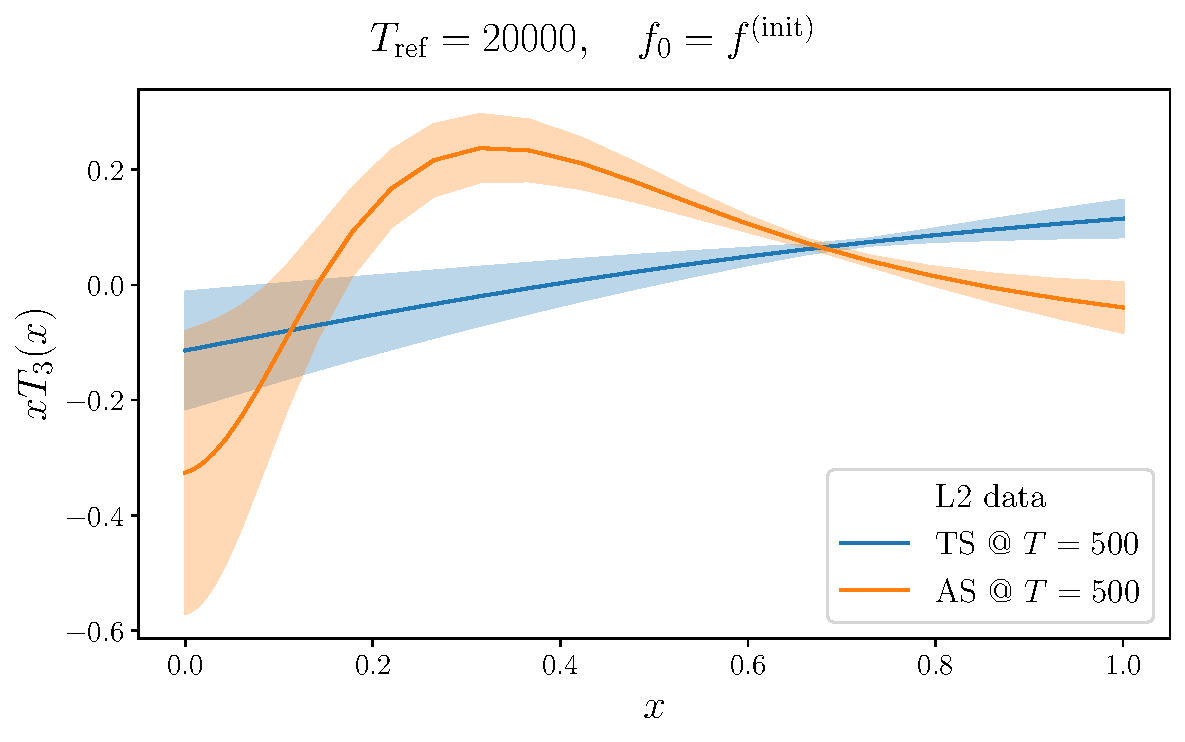
\includegraphics[width=0.45\textwidth]{plots/analytical_solution/xT3/evolution/tr_vs_an/L2/linear/evolution_vs_trained_epoch_500_L2_linear.pdf}
    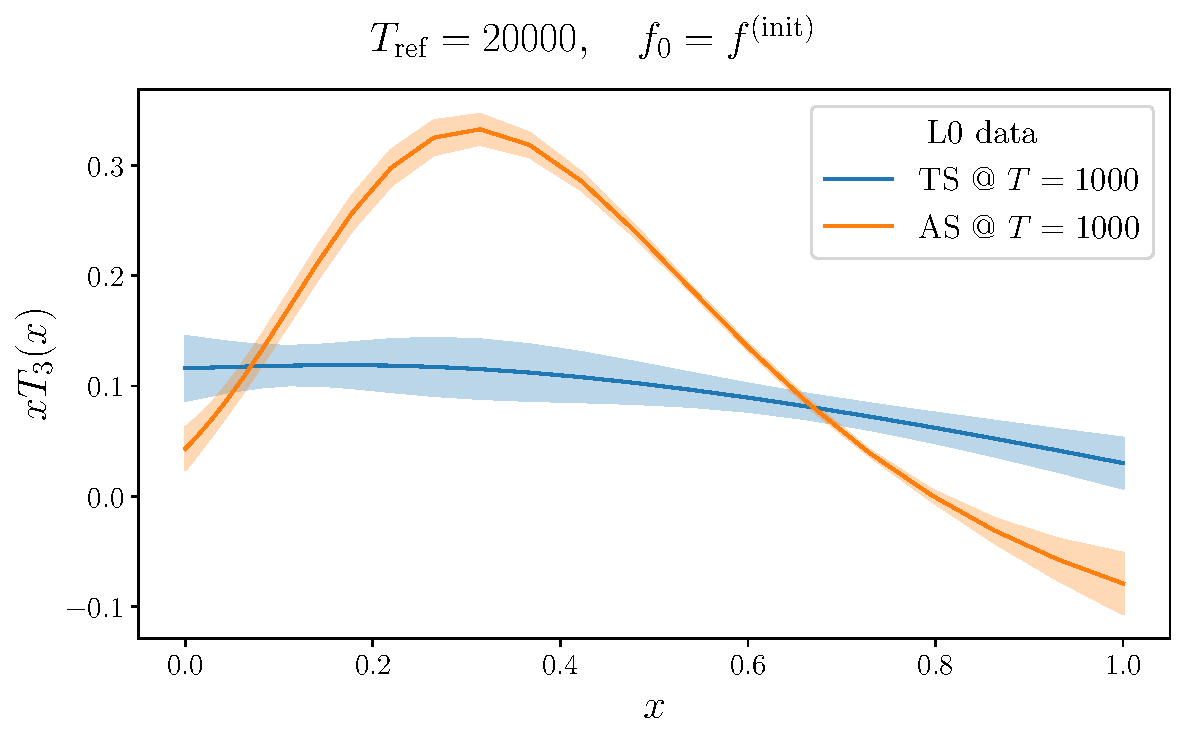
\includegraphics[width=0.45\textwidth]{plots/analytical_solution/xT3/evolution/tr_vs_an/L0/linear/evolution_vs_trained_epoch_1000_L0_linear.pdf}
    \hspace{10mm}
    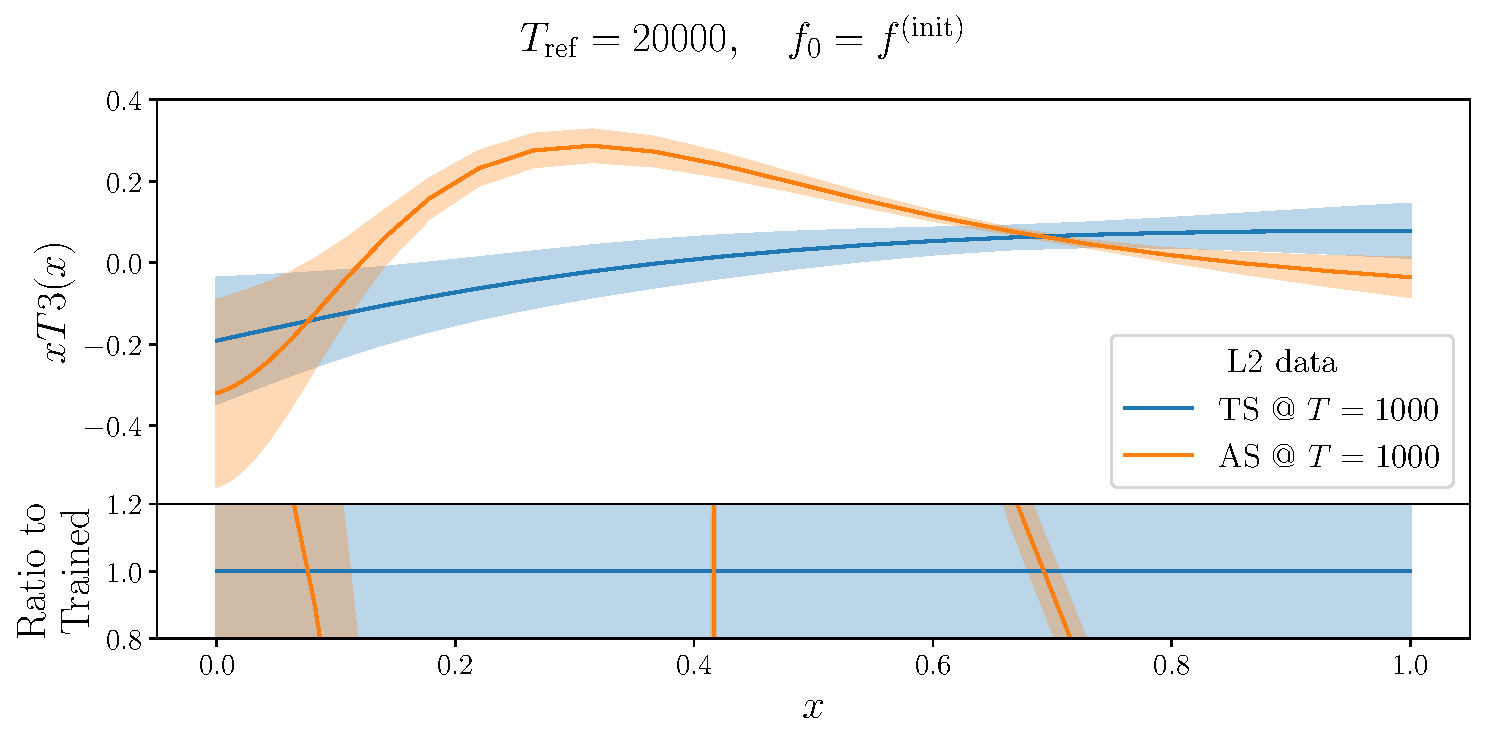
\includegraphics[width=0.45\textwidth]{plots/analytical_solution/xT3/evolution/tr_vs_an/L2/linear/evolution_vs_trained_epoch_1000_L2_linear.pdf}
    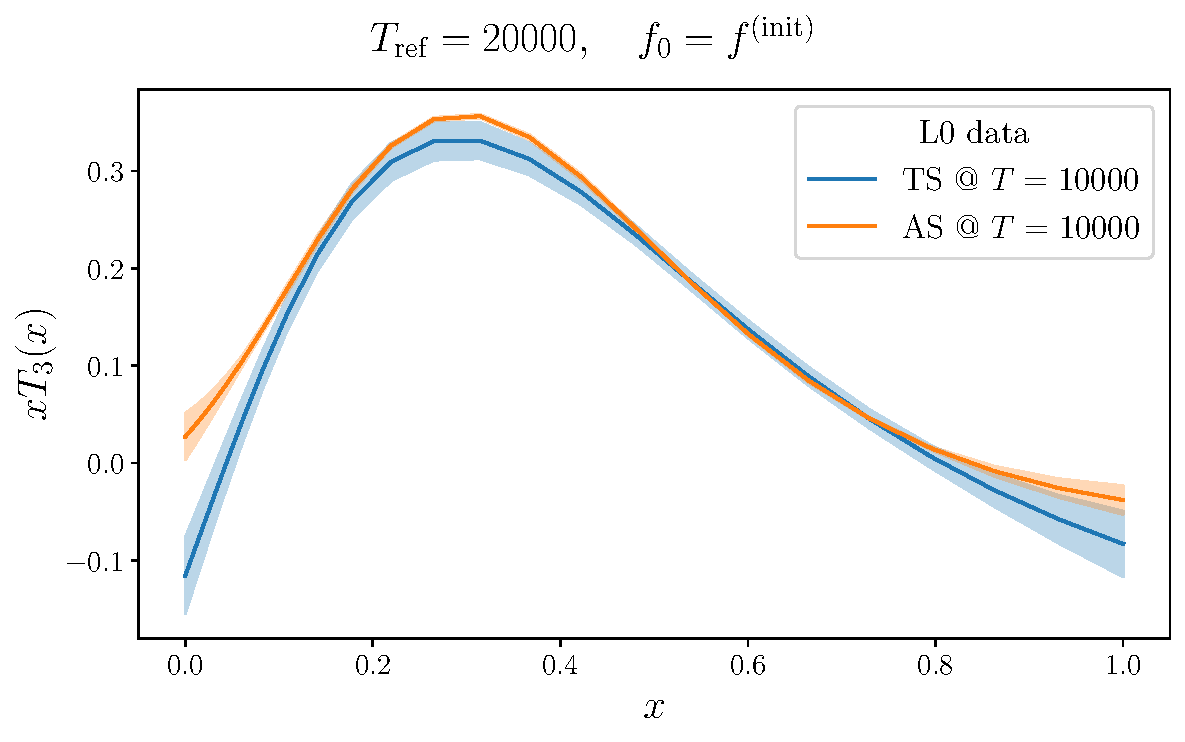
\includegraphics[width=0.45\textwidth]{plots/analytical_solution/xT3/evolution/tr_vs_an/L0/linear/evolution_vs_trained_epoch_10000_L0_linear.pdf}
    \hspace{10mm}
    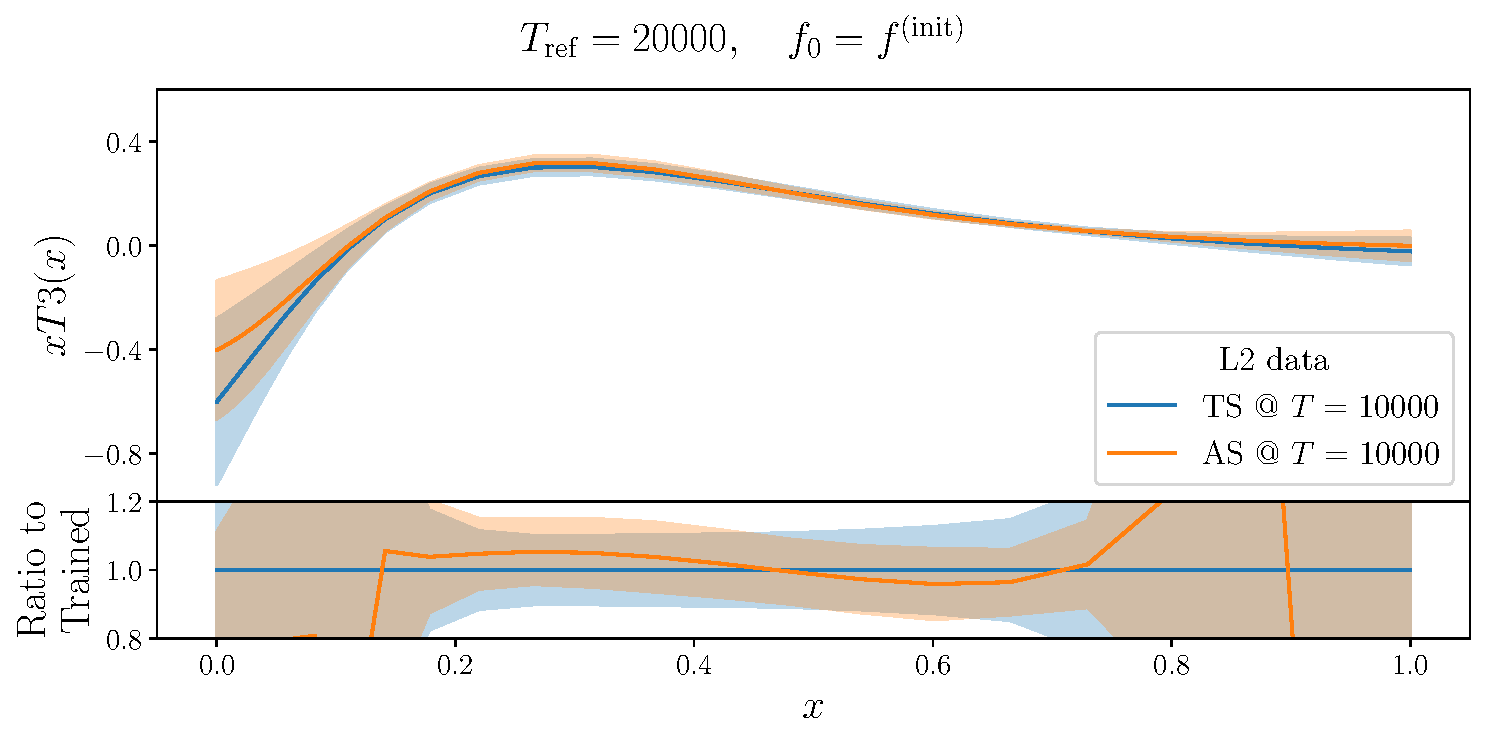
\includegraphics[width=0.45\textwidth]{plots/analytical_solution/xT3/evolution/tr_vs_an/L2/linear/evolution_vs_trained_epoch_10000_L2_linear.pdf}
    \caption{Comparison of the analytical solution and the trained solution at
    different epochs. The analytical solution is computed using the frozen NTK
    at $T_{\rm ref} = 20000$ and the initial function $f_0$ is a different
    ensemble of networks at initialisation. Left column shows results for L0
    data, while the right column shows results for L2 data.}
    \label{fig:xT3_analytical_vs_trained}
  \end{figure}
  % ===================================

% L0 data
\begin{figure}[ht!]
  \centering
  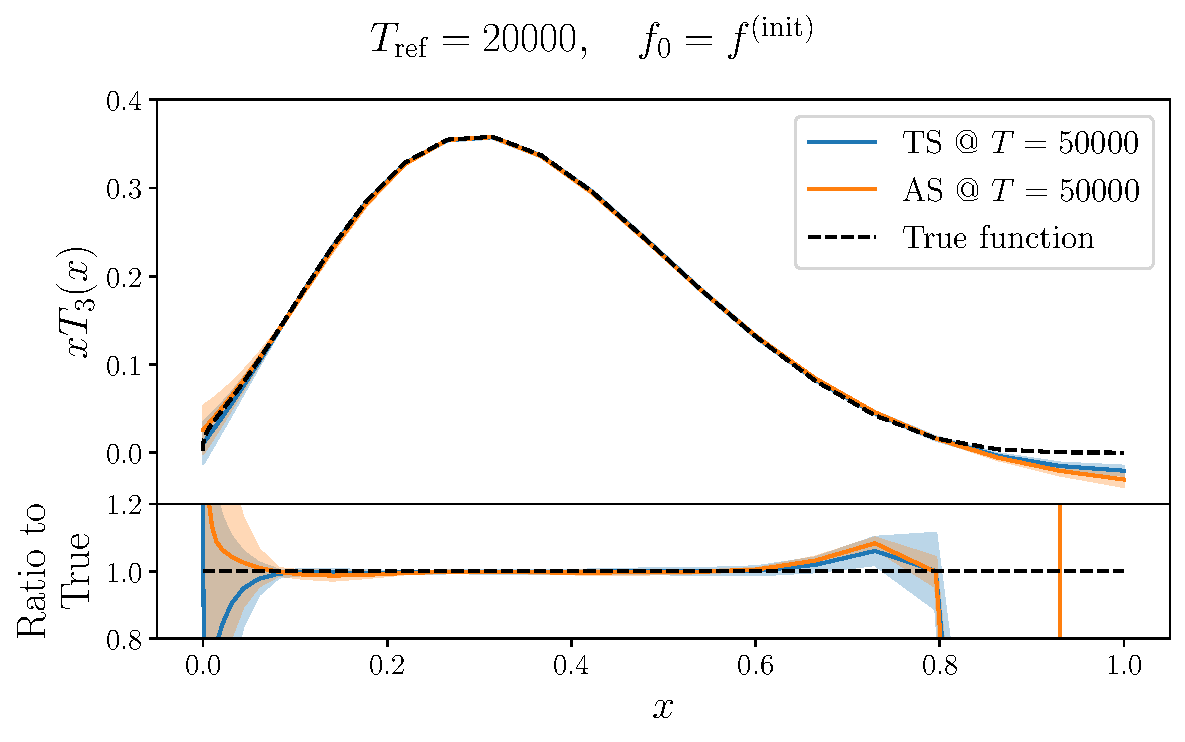
\includegraphics[width=0.48\textwidth]{plots/analytical_solution/xT3/evolution/from_f0/L0/linear/evolution_epoch_50000_L0_linear.pdf}
  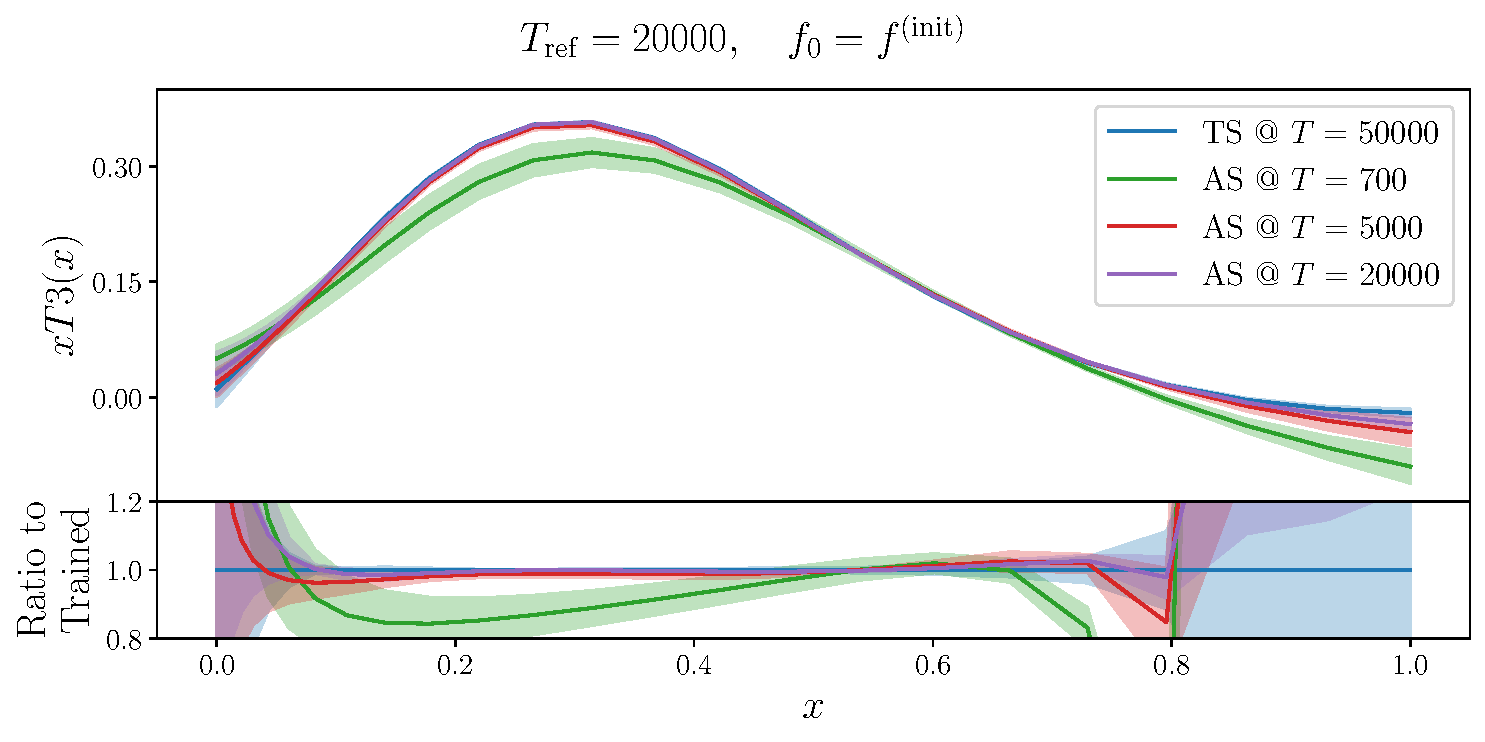
\includegraphics[width=0.48\textwidth]{plots/analytical_solution/xT3/evolution/from_f0/L0/linear/evolution_epochs_700_5000_20000_L0_linear.pdf}
  \caption{Comparison of the trained solution at the end of training and the
  analytical solution using L0 data. In both panels, the frozen NTK is chosen at
  $T_{\rm ref} = 20000$ and the initial function $f_0$ is a different ensemble
  of networks at initialisation. In the left panel, the analytical solution is
  evolved for $T_{\rm tot}$ epochs, while the right panel shows the same
  comparison for intermediate epochs.}
  \label{fig:xT3_analytical_init_L0}
\end{figure}
% ===================================

  % L2 data
\begin{figure}[ht!]
\centering
  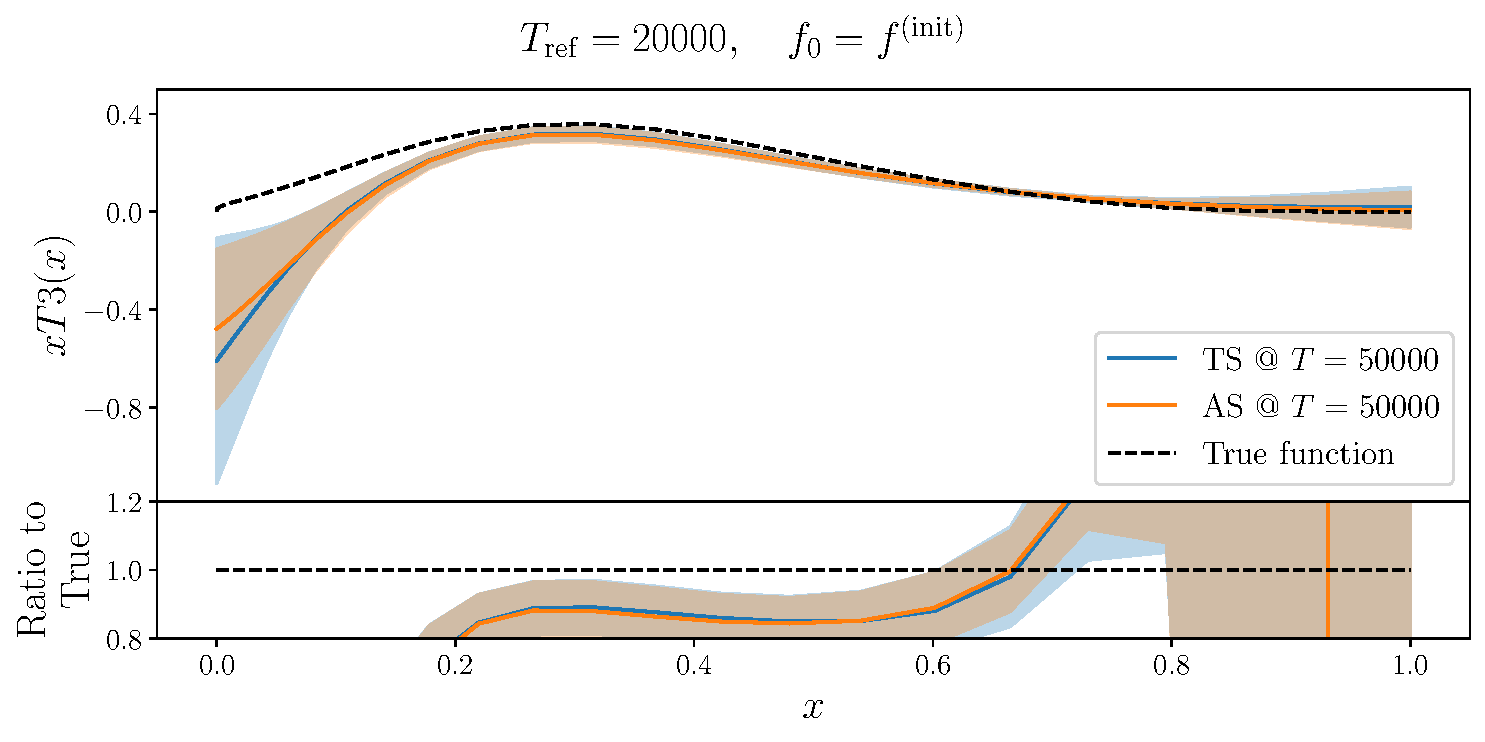
\includegraphics[width=0.48\textwidth]{plots/analytical_solution/xT3/evolution/from_f0/L2/linear/evolution_epoch_50000_L2_linear.pdf}
  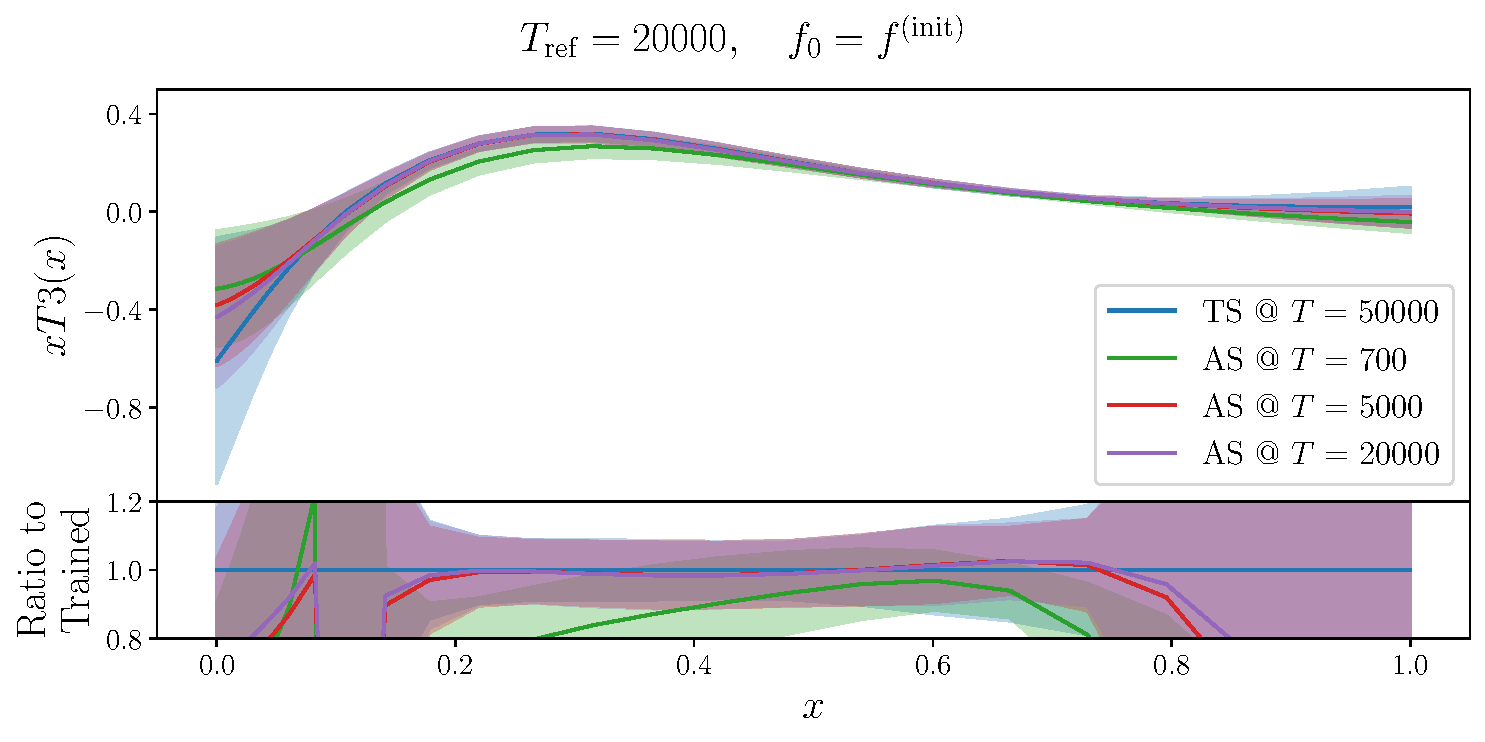
\includegraphics[width=0.48\textwidth]{plots/analytical_solution/xT3/evolution/from_f0/L2/linear/evolution_epochs_700_5000_20000_L2_linear.pdf}
\caption{Same as Fig.~\ref{fig:xT3_analytical_init_L0}, but using L2 data.}
\label{fig:xT3_analytical_init_L2}
\end{figure}

\FloatBarrier




  \begin{figure}[ht!]
    \centering
    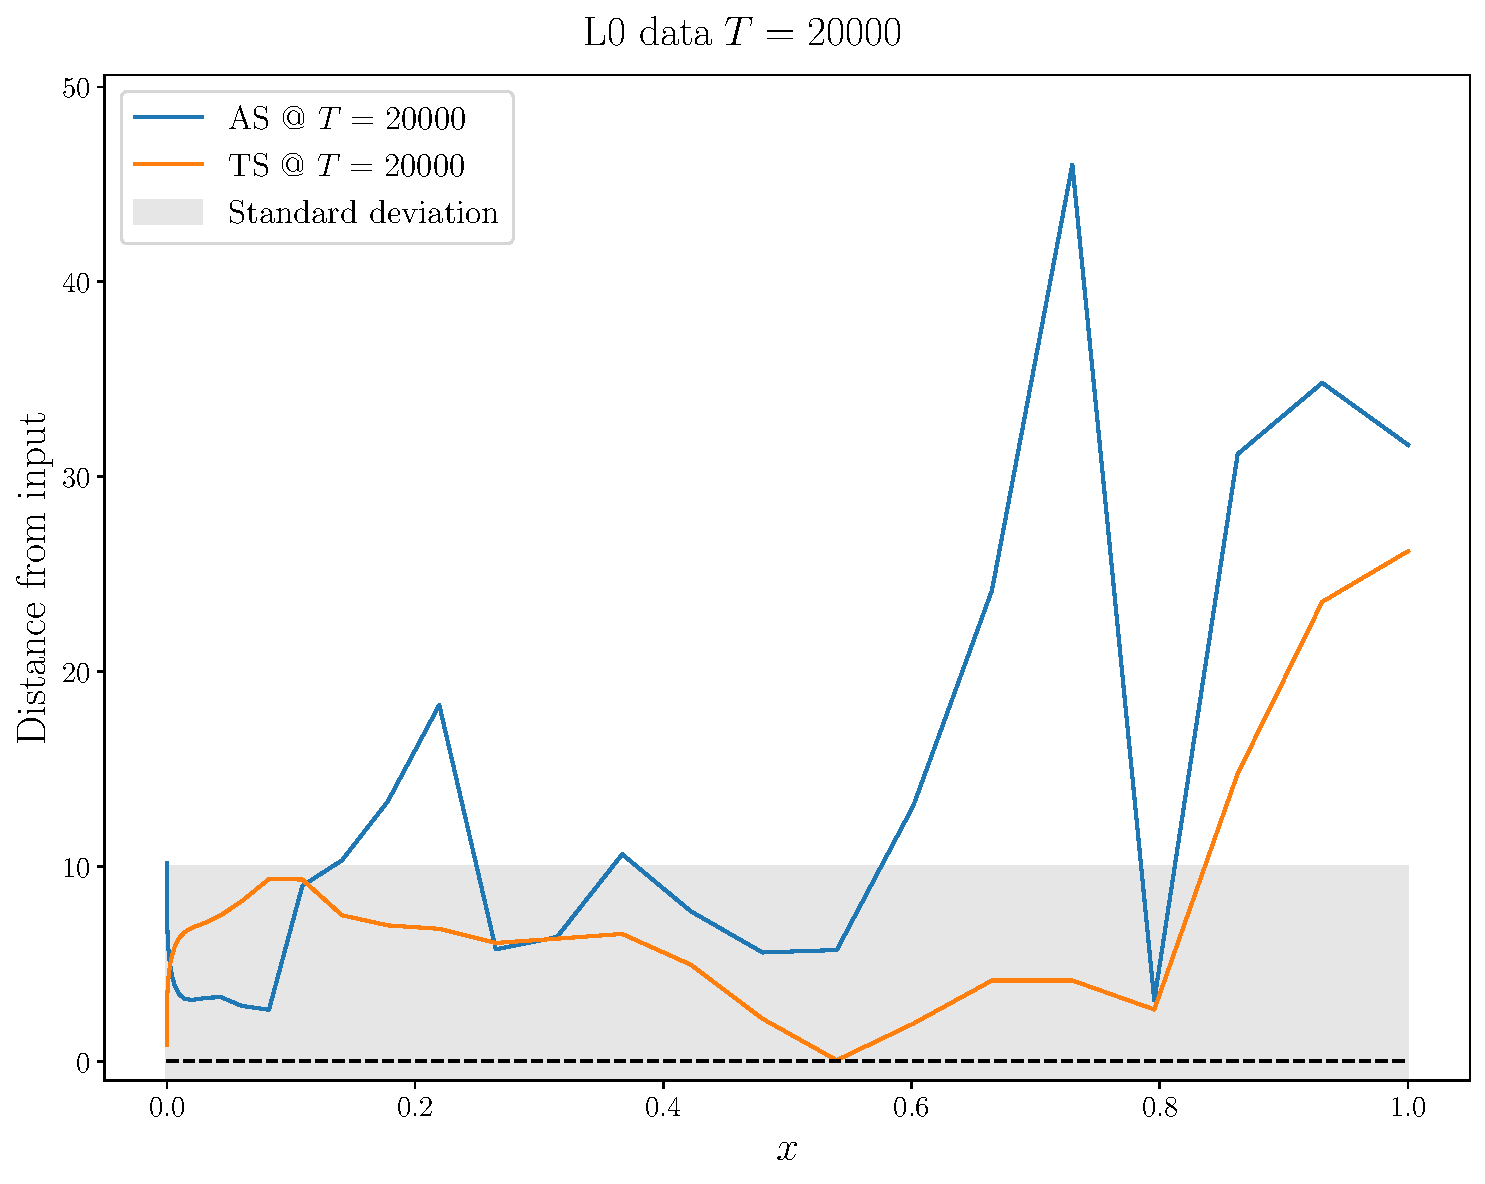
\includegraphics[width=0.48\textwidth]{plots/analytical_solution/xT3/distance_from_input/L0/linear/distance_from_input_epoch_20000_L0_linear.pdf}
    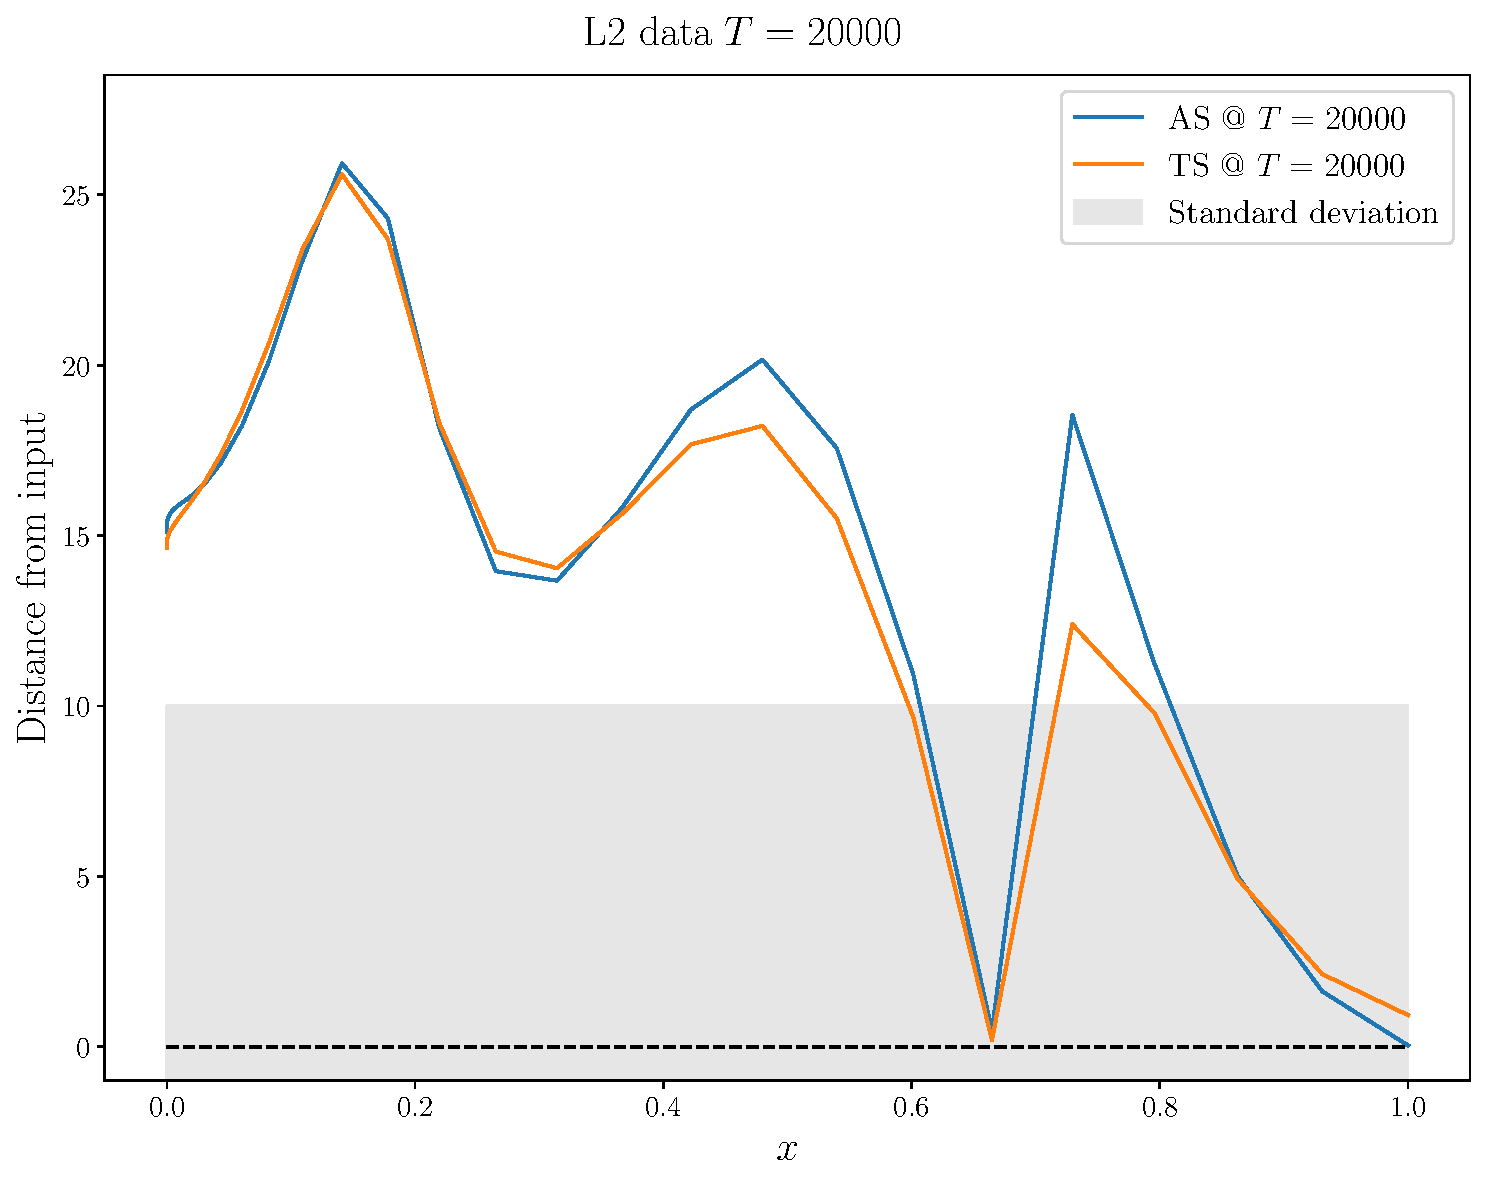
\includegraphics[width=0.48\textwidth]{plots/analytical_solution/xT3/distance_from_input/L2/linear/distance_from_input_epoch_20000_L2_linear.pdf}
    \caption{PDF distance, as defined in Ref.~\cite{NNPDF:2021njg}, with respect
    to the input function $\fin$ used to generate the data and the analytical
    and trained solutions in function of the evaluation epochs. The frozen NTK
    is chosen at $T_{\rm ref} = 20000$ and the initial function $f_0$ is a
    different ensemble of networks at initialisation. The left panel shows the
    case for L0 data, while the right panel shows the case for L2 data.}
    \label{fig:xT3_distance_L0_L2}
  \end{figure}
  % ===================================



\begin{figure}[ht!]
    \centering
    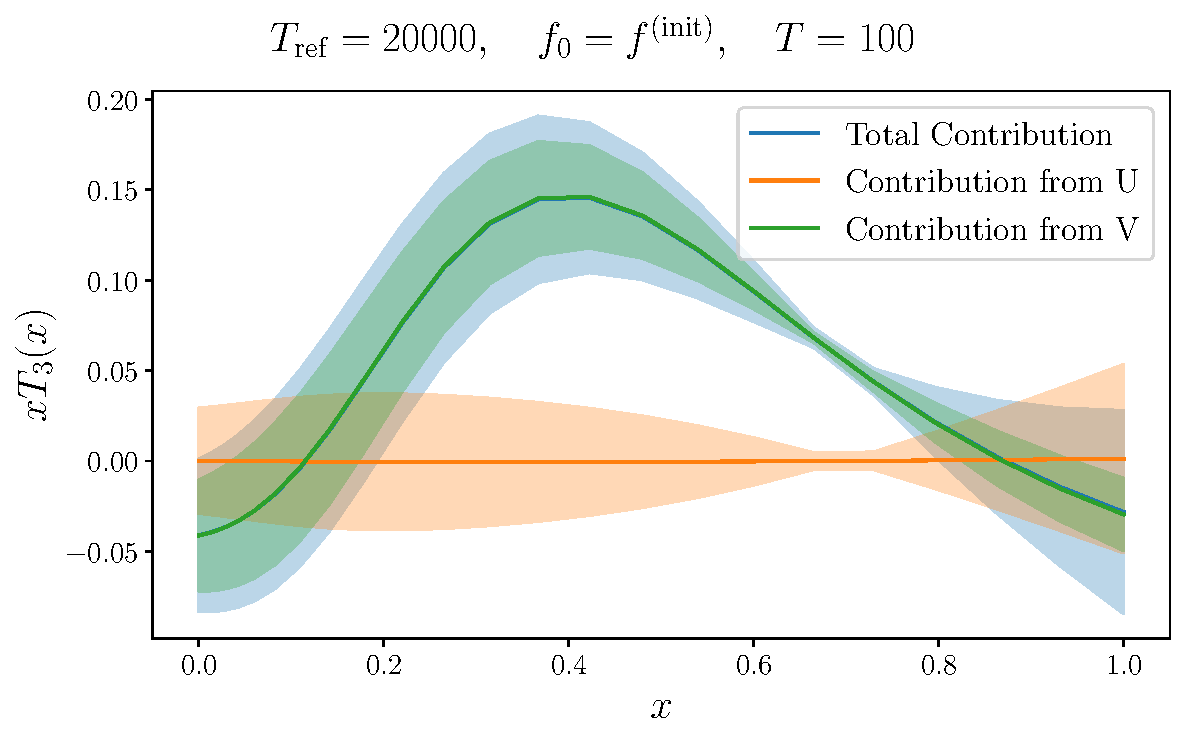
\includegraphics[width=0.45\textwidth]{plots/analytical_solution/xT3/u_v_decomposition/L0/linear/evolution_u_v_100_L0_linear.pdf}
    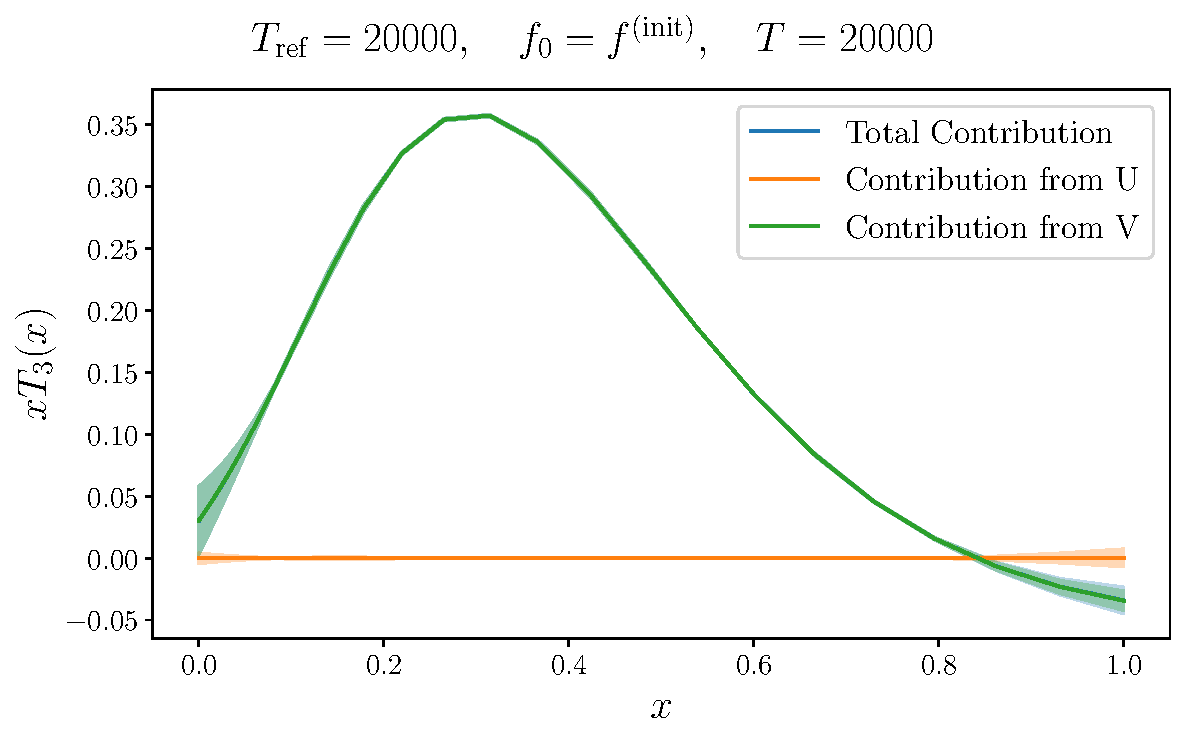
\includegraphics[width=0.45\textwidth]{plots/analytical_solution/xT3/u_v_decomposition/L0/linear/evolution_u_v_20000_L0_linear.pdf}
    \caption{Contribution of the $U$ and $V$ terms to the analytical solution.
    The left panel shows this breakdown at early stages of the analytical
    training ($T=100$ epochs); the right panel shows the contributions at the
    end of training, as in Fig.~\ref{fig:xT3_analytical_init_L0}.}
    \label{fig:xT3_u_v_contributions_L0}
  \end{figure}
  % ===================================

  \begin{figure}[ht!]
    \centering
    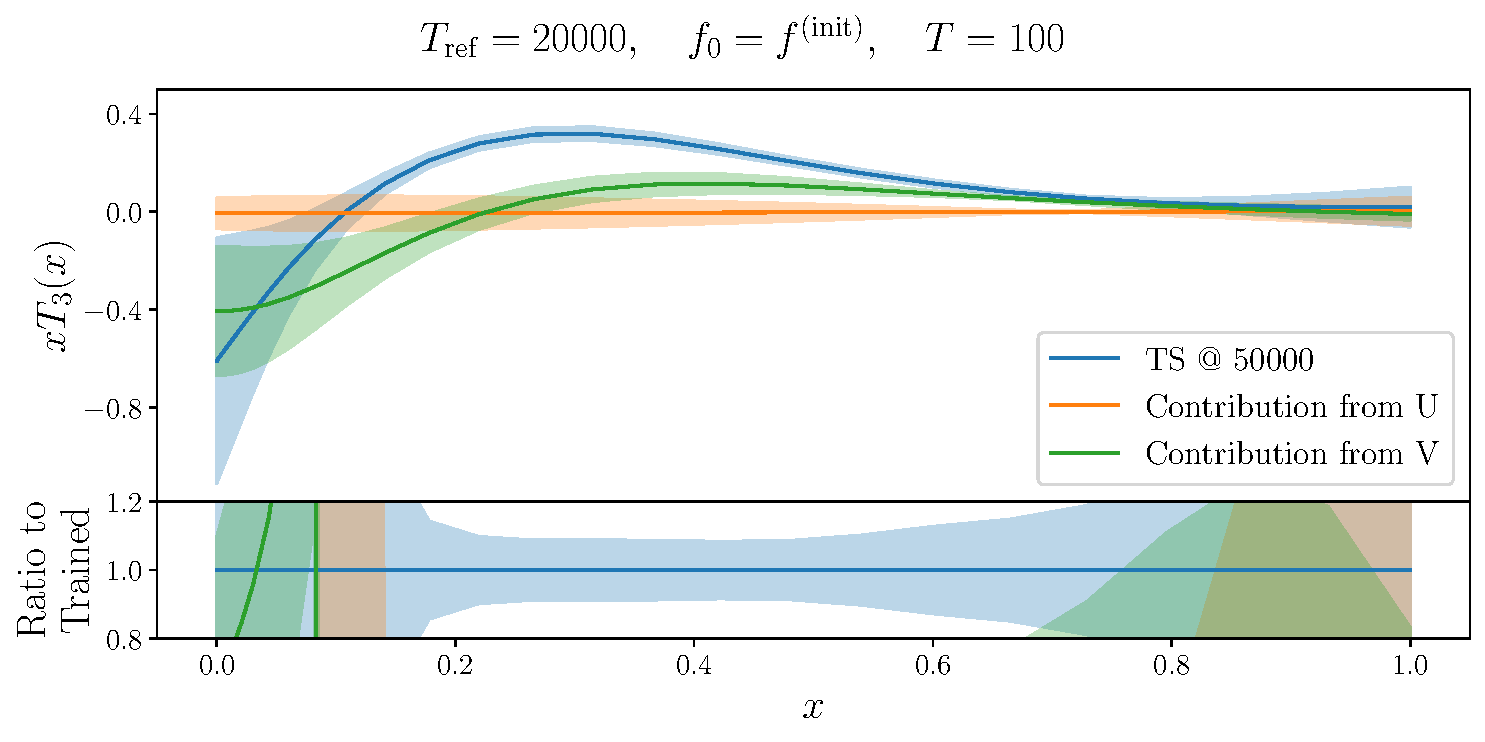
\includegraphics[width=0.45\textwidth]{plots/analytical_solution/xT3/u_v_decomposition/L2/linear/evolution_u_v_100_L2_linear.pdf}
    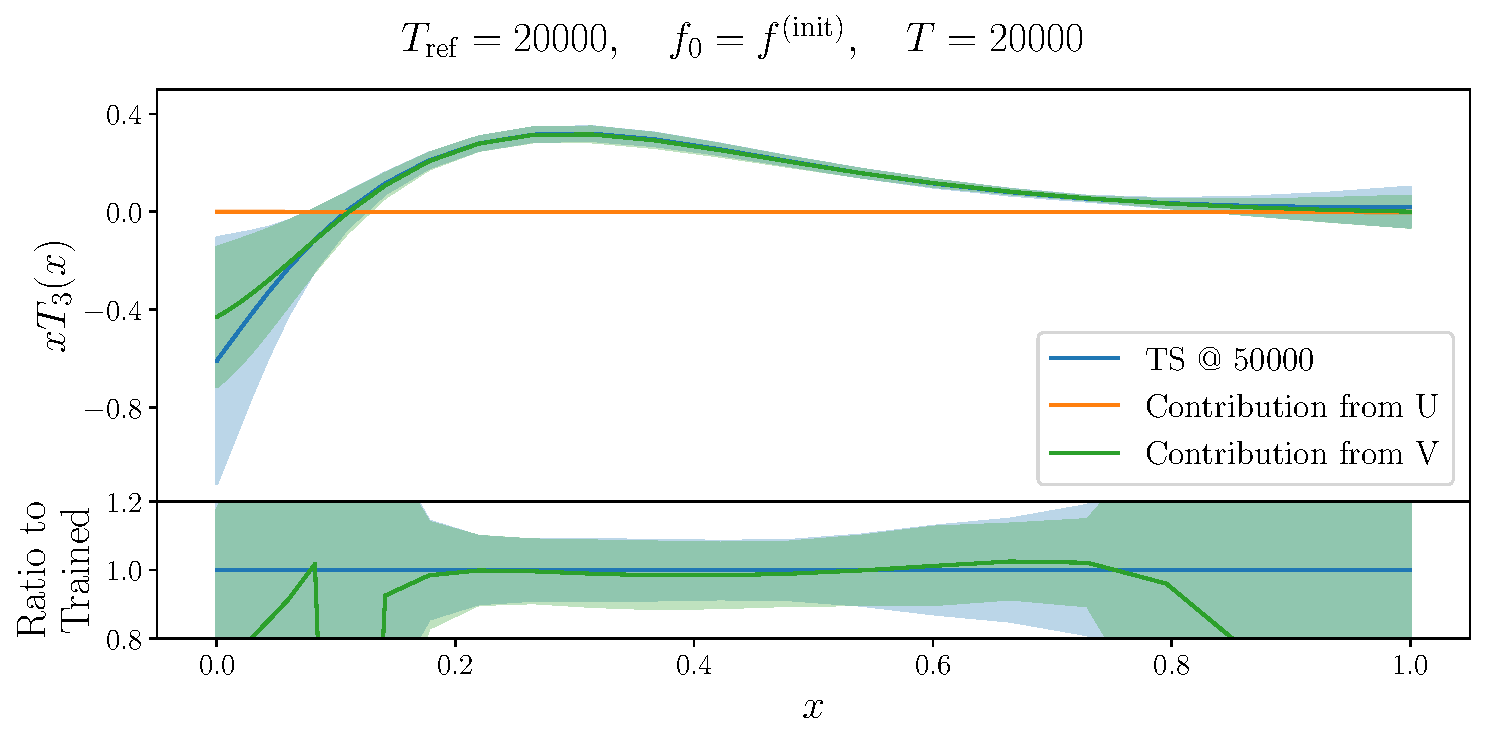
\includegraphics[width=0.45\textwidth]{plots/analytical_solution/xT3/u_v_decomposition/L2/linear/evolution_u_v_20000_L2_linear.pdf}
    \caption{Same as Fig.~\ref{fig:xT3_u_v_contributions_L0}, but using L2
    data.}
    \label{fig:xT3_u_v_contributions_L2}
  \end{figure}
  % ===================================

\FloatBarrier

\subsection{Covariance of the Analytical Solution}
\label{sec:CovarianceAnlyticalSolution}


% L0
% ===================================
\begin{figure}[ht!]
  \centering
  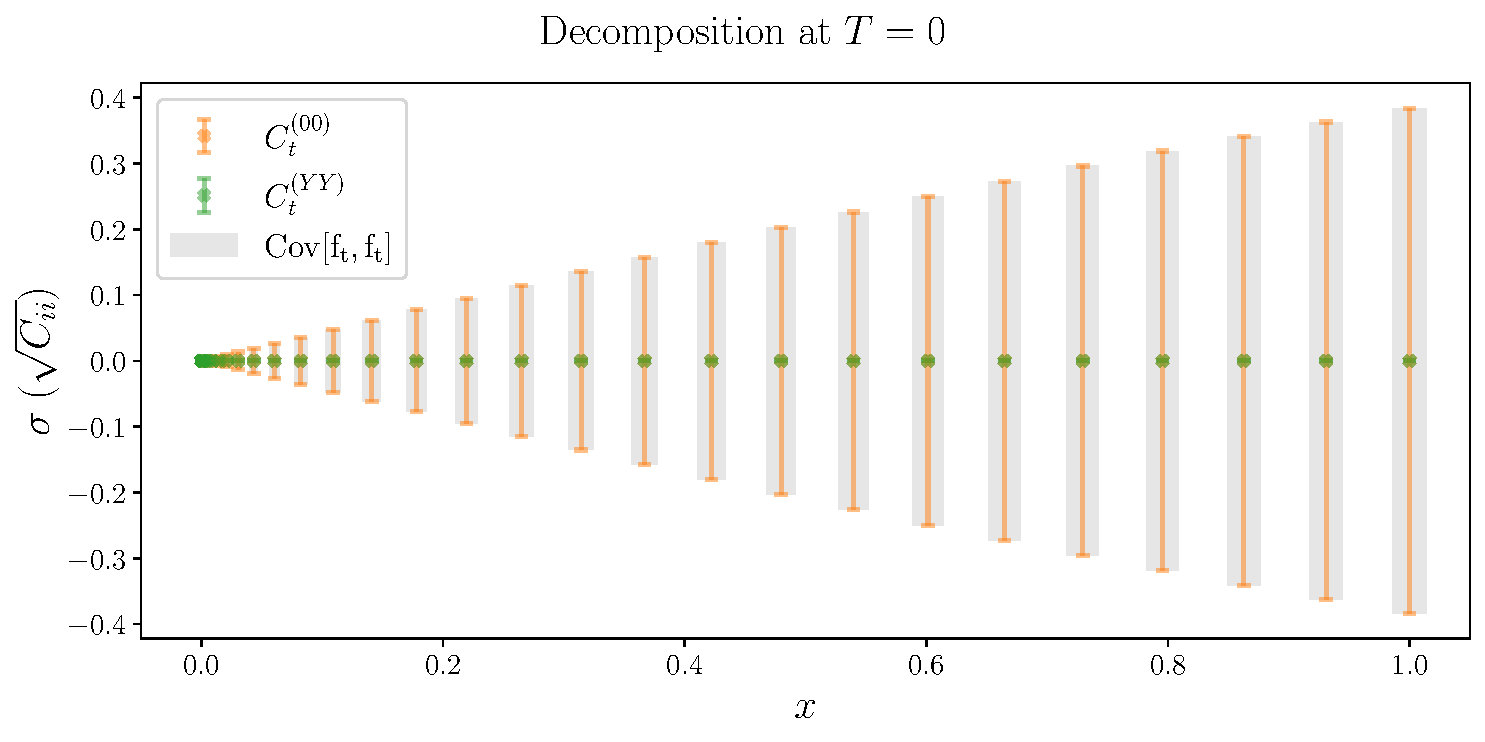
\includegraphics[width=0.32\textwidth]{plots/analytical_solution/xT3/covariance/diagonal/decomposition/L0/linear/diag_error_decomposition_epoch_0_L0_linear.pdf}
  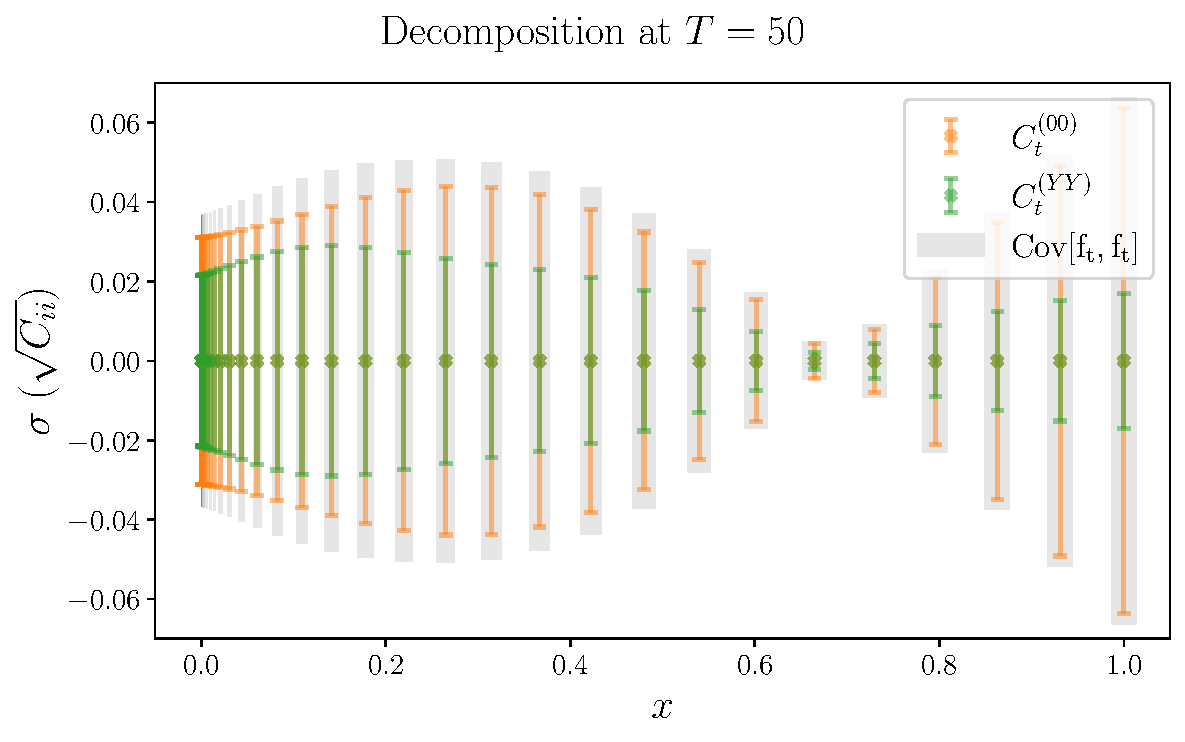
\includegraphics[width=0.32\textwidth]{plots/analytical_solution/xT3/covariance/diagonal/decomposition/L0/linear/diag_error_decomposition_epoch_50_L0_linear.pdf}
  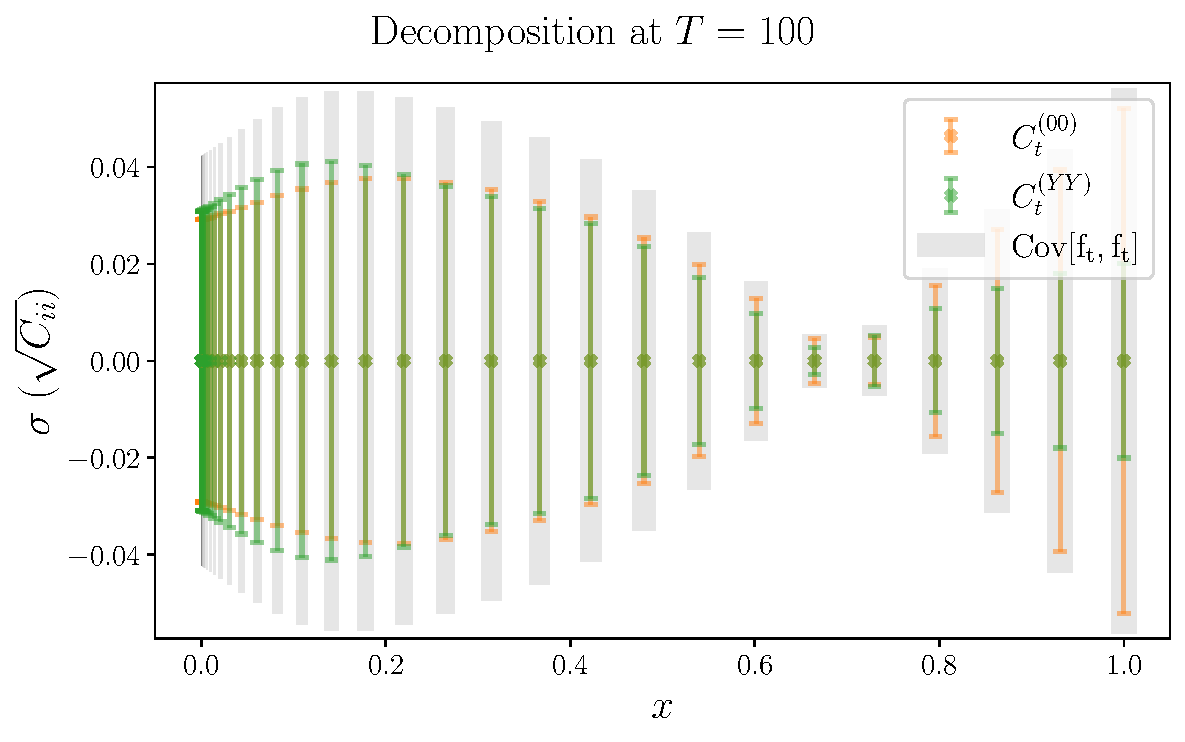
\includegraphics[width=0.32\textwidth]{plots/analytical_solution/xT3/covariance/diagonal/decomposition/L0/linear/diag_error_decomposition_epoch_100_L0_linear.pdf}
  \caption{Decomposition of the covariance of the analytical solution, as
  described in Eq.~\eqref{eq:SumOfCovariances}, for different training epochs.
  The square root of the diagonal elements is shown in the plots. The analytical
  solution is obtained by using a frozen NTK at $T_{\rm{ref}}=20000$ and the
  initial function $f_0$ is an ensemble of networks at initialisation different
  from the one used in the training process.}
  \label{fig:analytical_covariance_L0}
\end{figure}
% ===================================
% L2
% ===================================
\begin{figure}[ht!]
  \centering
  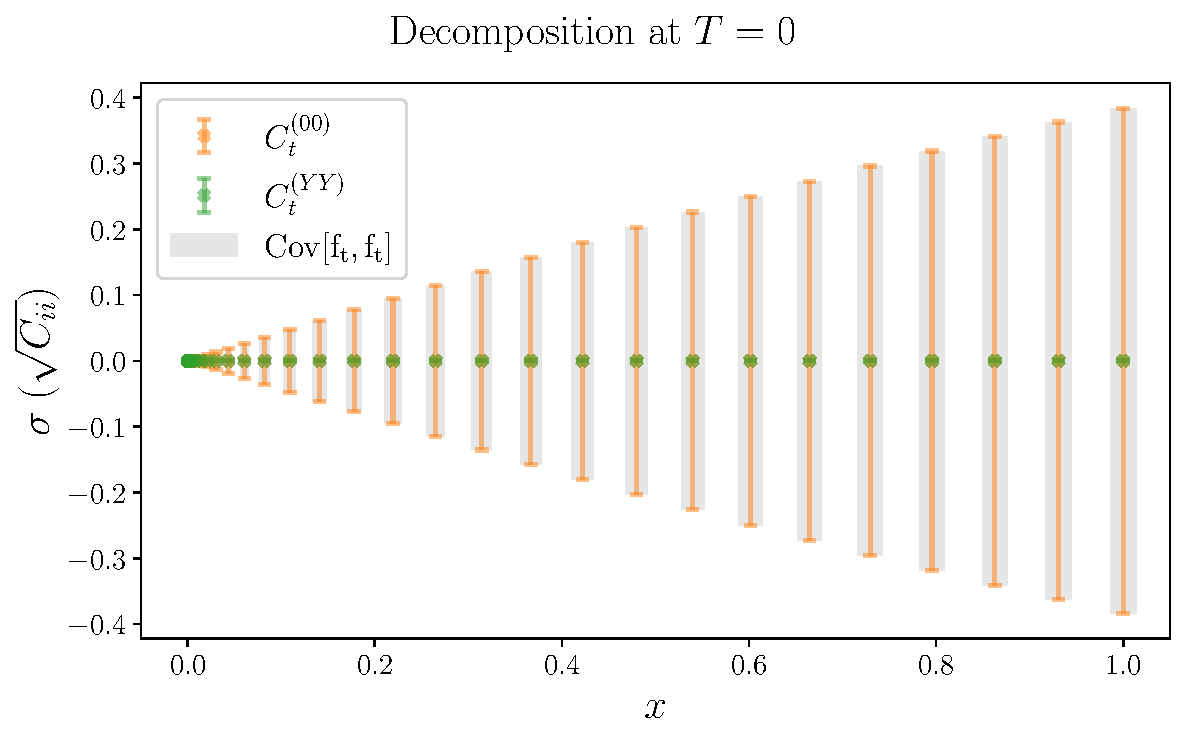
\includegraphics[width=0.32\textwidth]{plots/analytical_solution/xT3/covariance/diagonal/decomposition/L2/linear/diag_error_decomposition_epoch_0_L2_linear.pdf}
  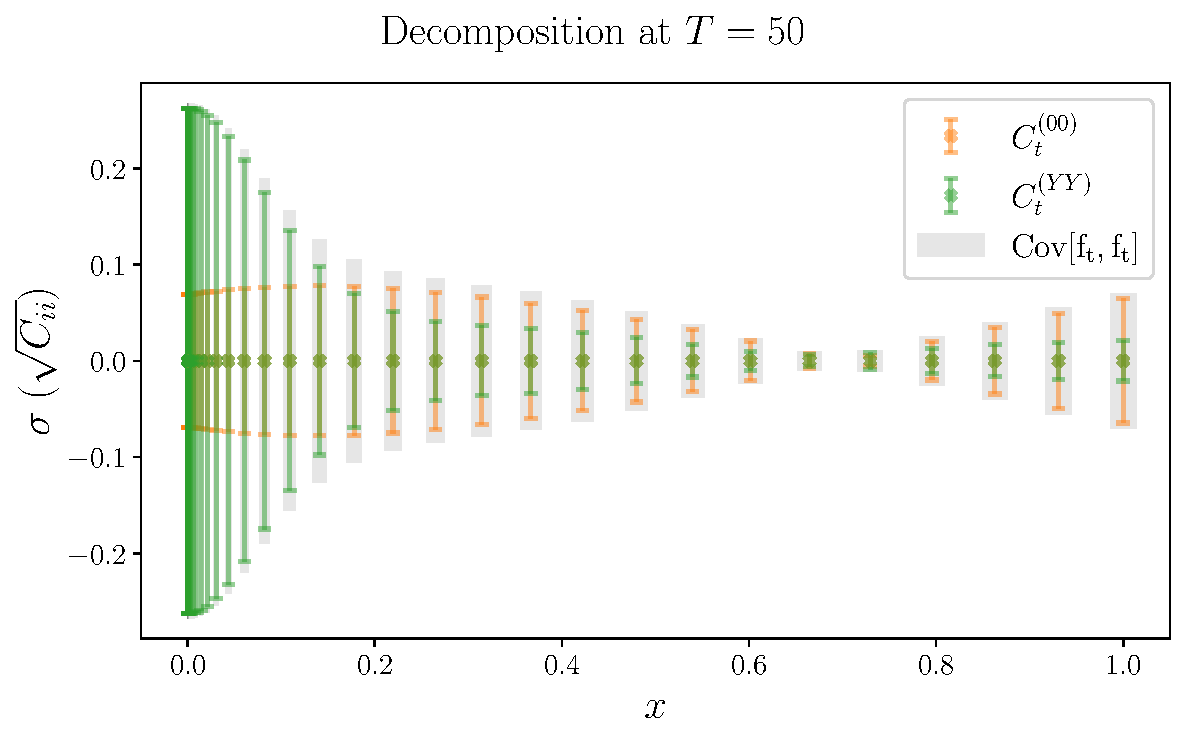
\includegraphics[width=0.32\textwidth]{plots/analytical_solution/xT3/covariance/diagonal/decomposition/L2/linear/diag_error_decomposition_epoch_50_L2_linear.pdf}
  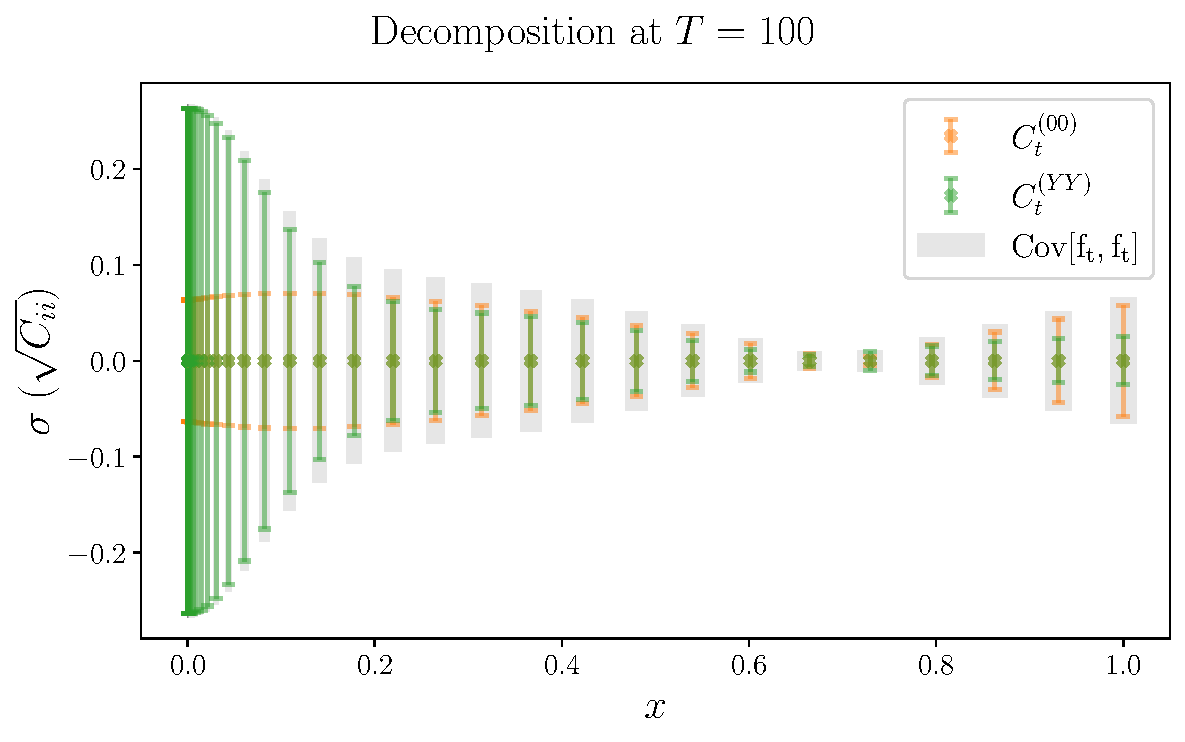
\includegraphics[width=0.32\textwidth]{plots/analytical_solution/xT3/covariance/diagonal/decomposition/L2/linear/diag_error_decomposition_epoch_100_L2_linear.pdf}
  \caption{Same as Fig.~\ref{fig:analytical_covariance_L0}, but for L2 data.}
  \label{fig:analytical_covariance_L2}
\end{figure}
% ===================================


An important criterion that we want to put forward at this point is that the
covariance of the trained fields should be dominated by the statistical error on
the data. This is the case towards the end of training as shown in Fig.~XXX. In
this way we ensure that the quoted error on the PDFs is actually dominated by
the statistical error on the data, and not by the fluctuations of the initial
fields. This is a crucial point, since it guarantees that the ensemble of
trained PDFs is not biased by the choice of prior that is made by selecting a
given architecture, activation function, and probability distribution for the
biases and weights at initialization. \ldd{More plots needed. To be discussed.}

\FloatBarrier
